\documentclass[12pt]{article} % font size


\usepackage{graphicx} % to include images
\usepackage{float} % to float figures
%\usepackage{booktabs,makecell} % for diagonal cells
%\usepackage{hyperref} % for hyperlinks
\usepackage{listings} % for including files
\usepackage[top=1in, bottom=1in, left=1.25in, right=1.25in]{geometry} % set margins
\usepackage{amssymb}
\usepackage{amsmath}
\usepackage{mathtools}
\renewcommand{\familydefault}{\sfdefault} % use sans serif per default
\usepackage{helvet} % use helvetica per default

\usepackage[utf8]{inputenc} % for unicode input characters
\usepackage[T1]{fontenc}

\lstset{%
  basicstyle=\scriptsize\sffamily,%
  commentstyle=\footnotesize\ttfamily,%
  frameround=trBL,
  frame=single,
  breaklines=true,
  showstringspaces=false,
  numbers=left,
  numberstyle=\tiny,
  numbersep=10pt,
  keywordstyle=\bf
}


\makeatletter

\makeatother
\usepackage[english]{babel}


\renewcommand{\familydefault}{\sfdefault} % use sans serif per default
\usepackage{helvet} % use helvetica per default

\usepackage[utf8]{inputenc} % for unicode input characters
\usepackage[T1]{fontenc}

\makeatletter

\makeatother

\begin{document}

\author{SID-LAKHDAR Riyane}
\title{Introduction to Cryptology and Coding\\ Lab 3: RSA coding}
\maketitle
\tableofcontents
\newpage


\section{Introduction}
This document resumes and explains the program that we have implemented for the 3rd lab of cryptology: RSA coding.   This program (attached to this document) may be run by simply running the two following commands (the parameters of this commands are optional):
\begin{itemize}
    \item make
    \item ./erathosten <Maximum number>
    \item ./trialDivision <Maximum number>
    \item ./millerRabin <Maximum number> <Threshold probability ($\in [0, 100]$)>
    \item ./RSA\_init <Key size in bits> <message to cipher>
\end{itemize}
To each question of the topic corresponds a specific executable, which will display the answer using a specific interface.\\








\section{Generating large prime numbers}
\subsection{Naive method}
To generate a prime number between $[2, n]$, we have implemented the two following functions:
\subsubsection{Eratosthenes sieve}
This functions is implemented within the file "largePrime\_naive.cc".\\  
It starts by randomly picking the rank r of the result prime number between $[0, \frac{n}{ln(n)}]$, where $\frac{n}{ln(n)}$ is a lower-bound of the number of prime numbers lower than n.\\
Then the function sequentially generates all the prime numbers until the rank r, using the Eratosthenes sieve.\\

This method aims to enumerate all the prime numbers until a sail n.   Thus for a given n, the number of prime that can be found is $\frac{n}{ln(n)}$.

Let s be the the size in memory a long integer (1 block of the type mpz).  For a given integer n, the number b of blocks used to store n, respects the relation:
\begin{equation}
\begin{aligned}
	2^{(b-1)*s}	& \leq n 						&<2^{b * s} \\
	b-1			& \leq \frac{ln(n)}{s * ln(2)}	&< b
\end{aligned}
\end{equation}
As this functions needs to go through all the positive integers until n (at most), the memory complexity of this algorithm is:\\
\begin{equation}
\begin{aligned}
	M(n) &= \sum_{i=1}^{n}{s*base(\frac{ln(i)}{s*ln(2)})}\\
    M(n) &= \frac{1}{ln(2)} * ln (n!)
\end{aligned}
\end{equation}
Where "base" is the function that associates to a double d the closest integer i which is less or equal d (see Figure \ref{memoryComplexity.pgm}).









\subsubsection{Trial division}
This functions is implemented within the file "largePrime\_naive.cc".\\  
It uses the same algorithm as previously to enumerate all the possible prime number until a randomly picked rank.   However, for a given integer n, the primality test used here is to compute the rest of the Euclidian's division of n by all the integer i such that $i < n$.   This test may be improved by only considering the odd integers i (and 2).\\

Thus, as for the previous question, for a given n, the number of prime that can be found is $\frac{n}{ln(n)}$.   And the memory complexity of this algorithm is: $M(n) = \frac{1}{ln(2)} * ln (n!)$ (see Figure \ref{memoryComplexity.pgm}).\\





\subsection{Miller\-Rabin based method}
\subsubsection{Base lemma}
\begin{itemize}
	\item Let prove that if n is prime then the only roots of the equation $x^{2} = 1 [n]$ are $x = 1$ and $x = -1$\\
        Let $x \in \mathbb{N}$ such that $x^{2} = 1 [n]$.\\
        Thus $\exists q \in \mathbb{N}$ such that
        \begin{equation}
        \begin{aligned}
            x^2				&= q*n + 1\\
            (x - 1) (x + 1) &= q*n
        \end{aligned}
        \end{equation}
        As n is prime, according to the Euclid's lemma, $n | (x-1)$ or $n | (x+1)$:
        \begin{itemize}
            \item if $n | (x-1)$, then $x = 1 [n]$
            \item if $n | (x+1)$, then $x = -1 [n]$
        \end{itemize}
        Thus the only solutions of the equation $x^{2} = 1 [n]$ are $x = 1$ and $x = -1$\\

    \item Let prove that if the only roots of the equation $x^{2} = 1 [n]$ are $x = 1$ and $x = -1$ then n is prime\\
\end{itemize}




\subsubsection{Primality base theorem}
According to Ferma's little theorem, as n is prime, $\forall m \in \mathbb{N}$ we have:
\begin{equation}
\begin{aligned}
	a ^ {n-1} &= 1 [n]\\
	a ^ {2^{s} *m } &= 1 [n]\\
\end{aligned}
\end{equation}

If $s = 0$, then $a^{m} = 1[n]$.  Otherwise
\begin{equation}
\begin{aligned}
	a ^ {2^{i}*2^{s-i} *m } &= 1 [n] \mbox{ with i } \in \{0, s\}\\
	(a ^ {2^{i} *m}) ^ {2^{s-i}} &= 1 [n]\\
\end{aligned}
\end{equation}
According to the previous result, $\exists$ s and m such that $a ^ {2^{i} *m} = -1$







\subsubsection{Miller\-Rabin witness algorithm}
To check if an integer a is the Miller-Rabin witness for the primality of an integer n, we have implemented the function "isMillerRabinWitness" within the file "largePrime\_millerRabin.cc".\\

This function starts by founding the couple $s, m$ such that $n-1 = 2^{s} * m$ where m is odd and s is the highest integer which respects this equality.   To do so, we simply loop over all the integers i until $2^{i} \neq 0 [n]$.   Thus it may be done with a complexity of at most $O(ln(n))$.\\

Then we iterate over all the $i \in {0, s-1}$ to check that $a^{2^{i} * m} \neq -1 [n]$.   Thus if we consider that a multiplication (modulo n) may be executed with a square complexity, then the complexity of our algorithm is:
\begin{equation}
\begin{aligned}
	C(n)	&= \sum_{i=1}^{s}{(\frac{ln(n)}{B * ln(2)})^{2}} \mbox{where B is the size of a block forming the mpz} \\
			&= s * (\frac{ln(n)}{B * ln(2)})^{2}\\
            &= O(ln(n) ^ {3}) \mbox{as s may be approximated by ln(n)}
\end{aligned}
\end{equation}
(see Figure \ref{memoryComplexity.pgm}).\\


\subsection{Memory complexity recap}
    \begin{figure}[!htb]\centering
	\begin{minipage}{0.8\textwidth} \frame{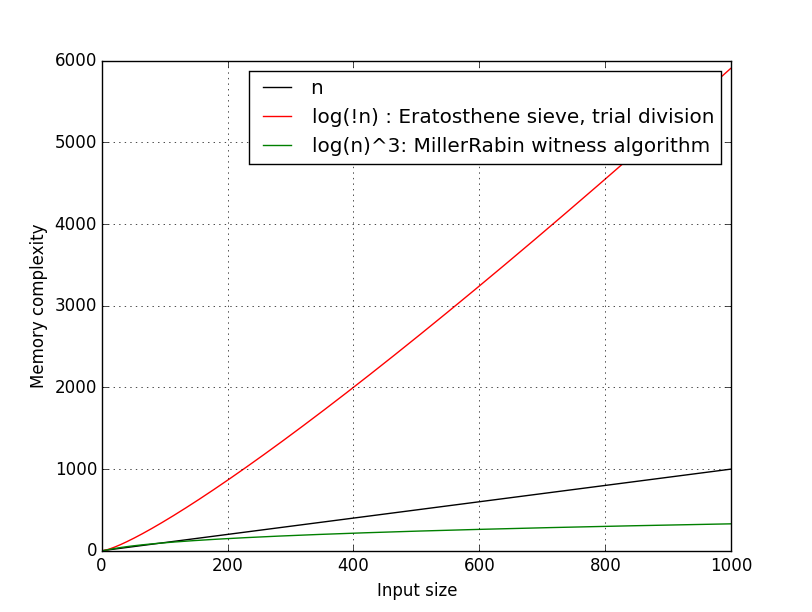
\includegraphics[width=\linewidth]{memoryComplexity.png}} \end{minipage}
	\caption{Memory complexity of the used algorithms}
	\label{memoryComplexity.pgm}
    \end{figure}



\section{RSA}
\subsection{Key generation}
The function that generates an RSA key has been implemented within the file "RSA\_init".\\
This function starts by generating two prime numbers (at the given order).   Then the function generates the public key e (encryption key) by randomly an integer $e < \phi(p*q)$ such that $e$ and $\phi(p*q)$ are relatively prime (where $\phi$ is the Euler's totient of $p*q$).   Finally, the function generate the private key d (decryption key) as the modular multiplicative inverse of $e$ modulo $\phi(p*q)$.

\subsection{Encryption, decryption}
The RSA encryption and decryption functions have been implemented within the file "RSA\_init".\\   It may be tested by runing the program "./RSA\_init" without parameters.  It may also been run by entering the parameters <key size (in bits)> <message>.
\end{document}